\section{Credit Market Implementation}

This model was adapted from the proposed model of the credit market
by the Ancona Unit. Here we present a description of how
the model was implemented.

\subsection{Description}
The credit market involves the interaction of the credit function
with the financial management functions of the Firm and Bank agent.
The state graph in Figure \ref{fig:statecredit} shows the flow of
activity in the model.

% \subsection{Agents}
% The agents involved in the implementation are listed below:
% \begin{itemize}
% \item Bank Agent - reads loans requests and approves loans.
% \item Firm Agent - requests for loans if needed.
% \item Dummy Agent - to handle message of orders and household
% functions.
% \end{itemize}
%
% \subsection{State dependency diagram}
%
% \begin{figure}[!htb]
% \begin{center}
%  \includegraphics*[scale=2.0]{stategraph.ps}
% \caption{State Dependency Diagram.} \label{fig:statecredit}
% \end{center}
% \end{figure}
%
% The state dependency diagram \ref{fig:statecredit} shows the flow of
% activity in the model. The details of the functions of the agents
% can be found in the report presented by the Ancona Unit \cite{?}.
%
% The xmml file for the credit market can be found in the Chapter
% \ref{appendix}.
%
% \section{Results}
% Graphs




\subsubsection{Firm Agent in the Credit Market}

See Table \ref{tab:creditbankfn}.

\begin{landscape}
\begin{table}[!htb]\caption{Functions being performed by the Firm involved in Credit Market.}
\begin{center}
\begin{tabular}{|c|c|c|l|c|c|}
\hline
Function Name & State From & State to & Condition on Function & Inputs & Outputs \\
\hline {\parbox[l]{3cm}{Firm \_ask \_loan}}& {\parbox[l]{3cm}{Start
\_Firm \_Credit \_Role}}& {\parbox[l]{3cm}{Firm \_Credit \_02}}&
{\parbox[l]{3cm}{a.external \_financial \_needs GT 0.0}} & &loan
\_request
\\
\hline

{\parbox[l]{3cm}{Firm \_get \_loan}}& {\parbox[l]{3cm}{Firm \_Credit
\_02}}& {\parbox[l]{3cm}{Firm \_End \_Credit \_Role}}&
&{\parbox[l]{3cm}{loan \_conditions ( a.id EQ m.firm\_id}} &
{\parbox[l]{3cm}{loan \_acceptance}}\\
\hline


\end{tabular}\end{center}\label{tab:creditbankfn}
\end{table}
\end{landscape}

\subsubsection{Bank Agent in the Credit Market}

See Table \ref{tab:creditbankmessages}.

\begin{landscape}
\begin{table}[!htb]\caption{Functions being performed by the Bank involved in Credit Market.}
\begin{center}
\begin{tabular}{|c|c|c|l|c|c|}
\hline
Function Name & State From & State to & Condition on Function & Inputs & Outputs\\
\hline

{\parbox[l]{3cm}{Bank \_decide \_credit \_conditions}} &
{\parbox[l]{3cm}{Bank \_start \_credit \_market \_role}} & Bank\_02
& & {\parbox[l]{3cm}{loan\_request (a.id EQ m.bank\_id)}} &
{\parbox[l]{3cm}{loan \_conditions}} \\

\hline

{\parbox[l]{3cm}{Bank \_give \_loan}} & Bank\_02 & Bank\_03 & &
{\parbox[l]{3cm}{loan \_acceptance (a.id EQ m.bank \_id)}} & \\

\hline

{\parbox[l]{3cm}{Bank \_receive \_instalment}} & Bank\_03 &
Bank\_04 & &
{\parbox[l]{3cm}{instalment (a.id EQ m.bank\_id)}} & \\

&&&&
{\parbox[l]{3cm}{bankruptcy (a.id EQ m.bank\_id)}} & \\

\hline


{\parbox[l]{3cm}{Bank \_account \_update \_deposits}} & Bank\_04 &
Bank\_05 & & {\parbox[l]{3cm}{bank\_account \_update (a.id EQ
m.bank\_id)}} &
{\parbox[l]{3cm}{central \_bank \_account \_update}}\\

\hline


{\parbox[l]{3cm}{Bank \_accounting}} & Bank\_05 &
{\parbox[l]{3cm}{end \_Bank \_cycle}} &
{\parbox[l]{4cm}{monthly (a.day \_of \_month \_to \_act)}}&  & \\

\hline


{\parbox[l]{3cm}{Bank\_idle}} & Bank\_05 & {\parbox[l]{3cm}{end
\_Bank \_cycle}} &
{\parbox[l]{4cm}{not (monthly (a.day \_of \_month \_to \_act))}}&  & \\
\hline


\end{tabular}\end{center}\label{tab:creditbankmessages}
\end{table}
\end{landscape}

\subsection{Messages being Used}

See Table \ref{tab:creditmarketmsg}.

\begin{table}[!htb]\caption{Messages involved in the credit market implementation.}
\begin{center}
\begin{tabular}{|c|l|l|}
\hline
Name & Variables being sent & Description \\
\hline loan\_request & {\parbox[l]{5cm}{firm\_id, bank\_id, equity,
total\_debt, external\_financial\_needs}}& {\parbox[l]{5cm}{Message
added by firm to demand credit with bank\_id,
with financial info of applying firm.}} \\
\hline loan\_conditions & {\parbox[l]{5cm}{firm\_id, bank\_id,
proposed\_interest\_rate, amount\_offered\_credit, value\_at\_risk}}
& {\parbox[l]{5cm}{Message added by bank to offer credit, contains
the interest rate, the amount of
offered credit, and the value\_at\_risk.}}  \\

\hline loan\_acceptance & {\parbox[l]{5cm}{bank\_id,
credit\_amount\_taken, loan\_total\_var}} & {\parbox[l]{5cm}{Message
added by firm to accept a loan with bank\_id, for the amount credit
taken and VAR. The bank
does not need to know the firm\_id.}}   \\
\hline

instalment & {\parbox[l]{5cm}{bank\_id, instalment\_amount,
interest\_amount, var\_per\_instalment}} & {\parbox[l]{5cm}{Message
added by firm pays
instalment and interest to the bank.}}    \\

\hline bankruptcy & {\parbox[l]{5cm}{bank\_id, bad\_debt,
credit\_refunded, residual\_var}} &{\parbox[l]{5cm}{Message added by
firm to bank
to signal bankruptcy.}}  \\
\hline BCE\_return &
{\parbox[l]{5cm}{bce\_debt, id}} & {\parbox[l]{5cm}{}}  \\
\hline

\end{tabular}\end{center}\label{tab:creditmarketmsg}
\end{table}


 \begin{figure}[!htb]
 \begin{center}
  \includegraphics*[scale=2.0]{stategraph.ps}
 \caption{State graph of the Credit Market Model.} \label{fig:statecredit}
 \end{center}
 \end{figure}

\subsection{Implementation Results}

The implementation of the agents described above was then simulated
to produce results which could later then be tested for verification
of the model. The results and technical details of the credit market
have also been discussed in D5.2.

The simulation consists of fifty iterations, that is 50 days. The
network is composted by $100$ firms and $10$ banks. Households are
replaced by the Dummy Agent.

Every month firms accomplish two main actions: they ask for loans
and pay debt installments, inclusive of interests. The demand of
credit occurs once per month. All firms, for sake of simplicity, are
activated in the first day of each month. Interests are payed back
every day after the loan has been taken out. The more relevant
initial conditions of firms have been set as follows: $equity=100$,
\emph{total debt=0}, $cash=100$ and \emph {total assets=0}.

As far as banks are concerned, they have the task to lend money and
fix interest rates whenever required by firms. Then, banks collect
interests and installments payed back by firms increasing, so, their
equity and cash. At the end of the month, banks with positive
profits will pay taxes and dividends. \\Relevant bank variables have
the following initial values:  \emph{cash=1000}, \emph{total
credit=0}, \emph{equity=1000}, \emph{debts versus BCE=0},
$\gamma_t$=0.2, $\gamma_{t-1}$=0.4, \emph{BCE's interest 2\%},
$\alpha$=0.8 and $\pi_{t-1} = \pi_{t-2}$=500.

Figure (\ref{fig:equity}) shows the average bank equity along the
simulation time. In the first twenty days it increases thanks to
interest payments. In the first day of the second month ($21^{st}$
iteration), banks pay taxes and, so, the equity shrinks. Then, since
banks grant new loans and, consequently, new interests are payed,
the everage equity increases again and so on. It is worthwhile to
note that in the second month equity grows less because banks are
short of liquidity and lend less money. This is because we have not
considered deposits from households (which are created in another
\emph{EURACE} module); additional liquidity, disposable for new
loans, comes only from firms' payment of installments relative to
previously contracted debts.


\begin{figure}[h!]
% \vskip 2cm
%  \centerline{
%   \epsfxsize 7cm \epsffile{equity.pdf} \hskip .5cm}
 \begin{center}
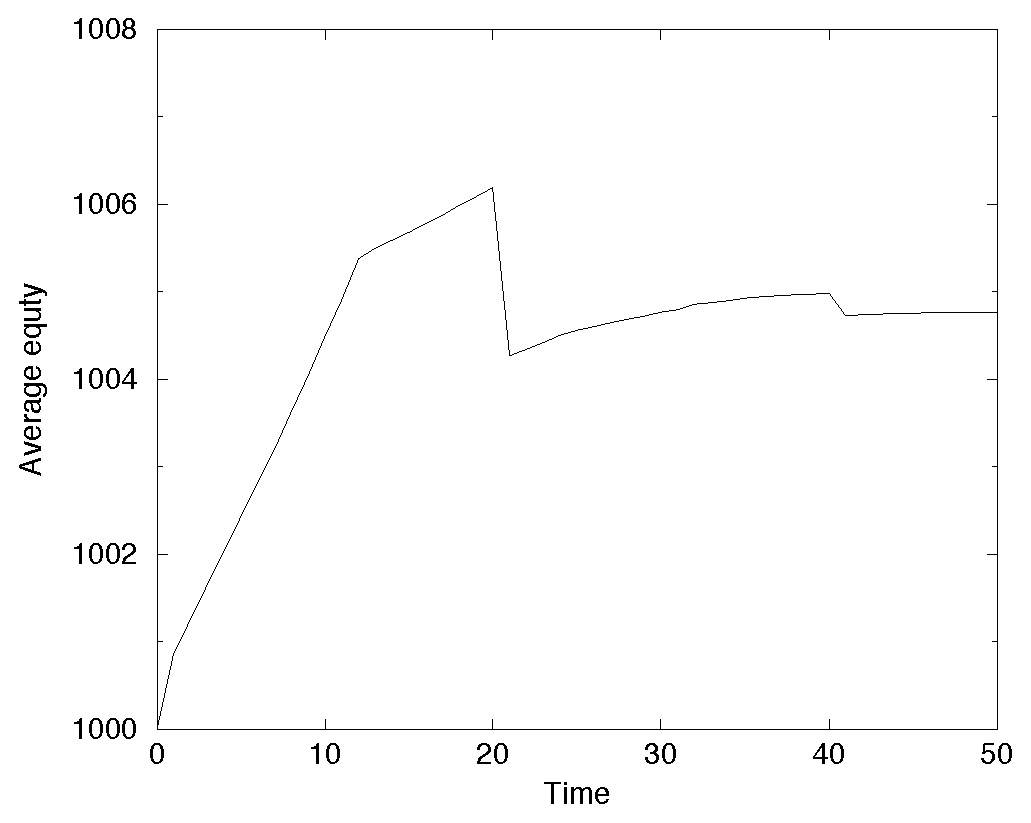
\includegraphics{equity.eps}
  \caption{Time series of average bank equity. Jumps occur when taxes are payed.}
 \label{fig:equity}
  \end{center}
\end{figure}


In figure (\ref{fig:data-bankave}) we can see the average bank cash.
After the first period it decreases abruptly because of loan demands
occurring in the same time. In the following days, banks receive
installments and can build up their liquidity again. The same
reasoning for equity applies: we do not have deposits, so cash can
only re-establish slowly and is immediately absorbed by new credit
demands: that is why the average cash shows along time only small
increases.

\begin{figure}[htb]
% \vskip 2cm
% \centerline{
%  \epsfxsize 7cm \epsffile{data-bankave.pdf} \hskip .5cm}
 \begin{center}
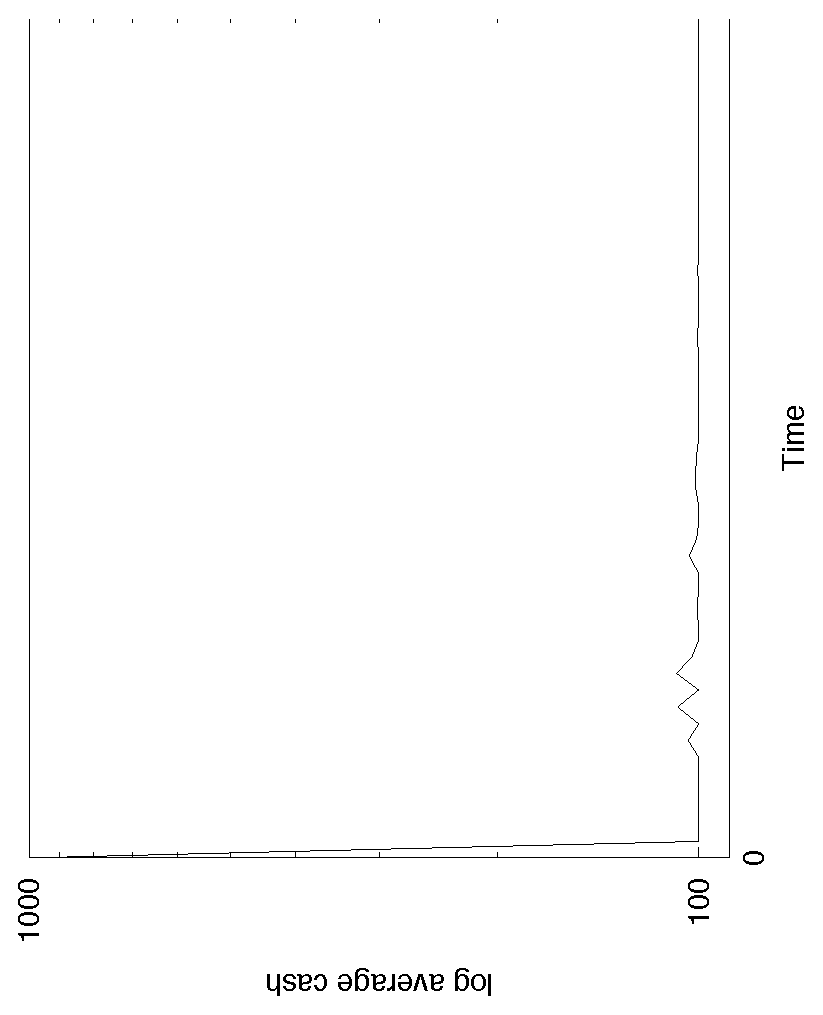
\includegraphics[angle=-90]{data-bankave.eps}
 \caption{Time series of average bank liquidity supply.}
 \label{fig:data-bankave}
   \end{center}
\end{figure}
